\subsection{Traffic Demand Per Subscriber}\label{subsec:behavior}

\begin{figure}[t]
\begin{minipage}{1\linewidth}
\centering
%
\begin{subfigure}[b]{1\linewidth}
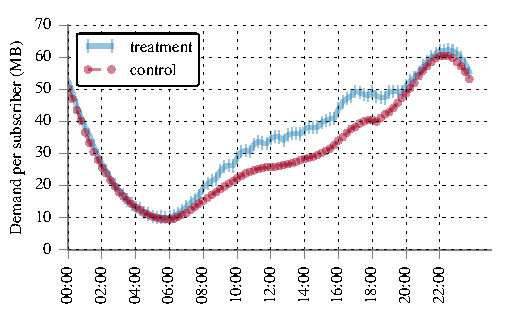
\includegraphics[width=\linewidth]{figures/weekday_demand_mean.pdf}
               \caption{Weekday traffic demand\label{fig:weekday-daily-usage}}
\end{subfigure}
%
\begin{subfigure}[b]{1\linewidth}
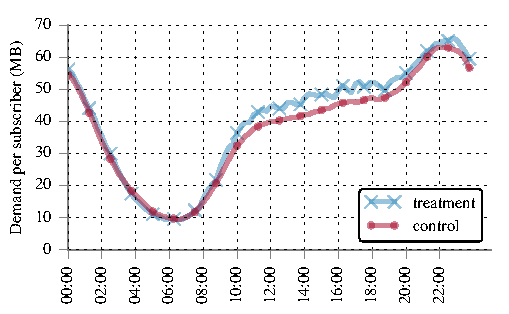
\includegraphics[width=\linewidth]{figures/weekend_demand_mean.pdf}
               \caption{Weekend traffic demand\label{fig:weekend-daily-usage}}
\end{subfigure}
%
\end{minipage}
\caption{Average subscriber demand (bytes every 15-minutes)}
\label{fig:traffic-demand-timeseries}
\end{figure}

Figure \ref{fig:traffic-demand-timeseries} shows the downlink traffic demand
(bytes per 15 minutes) of an average subscriber over a week.
We observe that subscriber behavior differs
significantly on weekdays and weekends. On weekdays, traffic demand 
increases monotonically from morning until prime-time hours in the evening. On 
weekends, we observed a sharp rise in demand in the early morning period, from
8:00 AM to 10:00 AM. Then, the demand plateaued until the next rise during before
evening prime-time hours. Previous reports indicate that the aggregate traffic volume
for US fixed access link providers usually troughs during mid-afternoon hours 
(between 2:00 PM -- 6:00 PM)~\cite{sandvine20141h}. We do not observe such troughs
in the subscriber demand in our dataset.

\begin{figure}[t]
\begin{minipage}{1\linewidth}
\centering
%
%\begin{subfigure}[b]{.33\linewidth}
%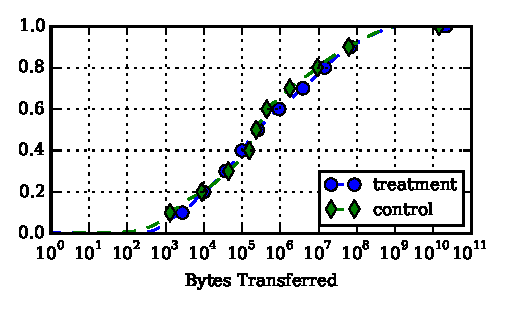
\includegraphics[width=\linewidth]{figures/cdf-all-bytes.pdf}
%                \caption{Overall traffic demand for all subscribers at all times\label{fig:CDF-data-rate}}
%\end{subfigure}
% maybe should be mean per day?
%
\begin{subfigure}[b]{1\linewidth}
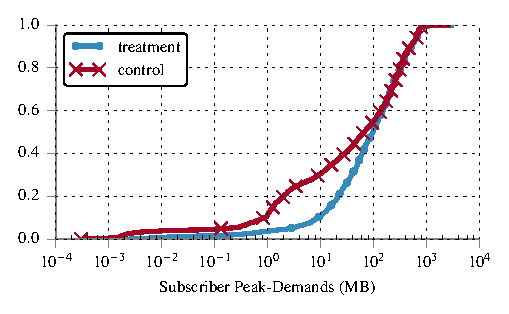
\includegraphics[width=\linewidth]{figures/cdf_peak_demand-overall.pdf}
               \caption{Peak (95\%) traffic demand per subscriber\label{fig:CDF-data-rate-perc95}}
\end{subfigure}

\begin{subfigure}[b]{1\linewidth}
% 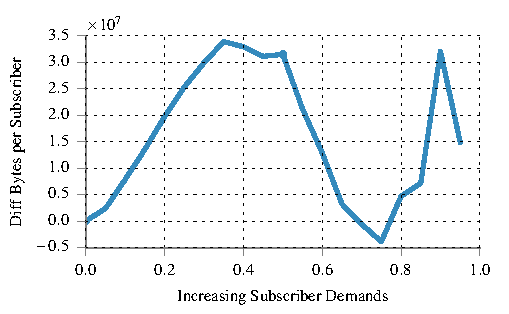
\includegraphics[width=\linewidth]{figures/diff_perc95_bytes_subsc-overall.pdf}	% 5 percentile
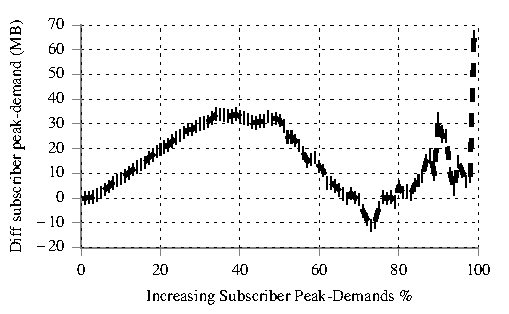
\includegraphics[width=\linewidth]{figures/diff_perc95_bytes_subsc-overall_01.pdf}		% 1 percentile
               \caption{Difference in overall peak per subscriber\label{fig:diff-peak-overall}}
\end{subfigure}
%
\end{minipage}
\caption{95th percentile traffic demand (bytes every 15-minutes) per subscriber for \control{} and \treatment{}\label{fig:traffic-demand-overall}}
\end{figure}

% Figure \ref{CDF-data-rate} shows the data rate for each measurement period and every subscriber.
Figure \ref{fig:CDF-data-rate-perc95} shows the distribution of the
the 95th percentile downlink traffic demand 
over the three month measurement period. The highest peak
demand amongst subscribers in the lower tier was 2.97 GB,
and 3.0 GB in the higher tier.

The average peak traffic demand was 169.8 MB for \control{} and
186.6 MB for \treatment{}. Given the 105 Mbps service tier capacity,
this means that users even on averaging the 95th percentile demand,
users rarely utilize their links (average utilization was 1.43\%
for \control{} and 1.5\% for \treatment{})

Similar to previous studies, we suspected that the subscribers downloading most bytes
by volume on the higher tier link would be the ones causing the largest difference
in mean demand. However we observed that the median peak demand 
was 66.7 MB for the lower tier, and 98.4 MB for the higher tier
showing a clear increase in demand in the upgraded service tier
group. We found that, the difference in the average peak demand
was also preset in the lowest demanding 50\% subscribers
in the control group, when compared to the lowest demanding subscribers of the treatment
group. This shows up as a large gap under the 50\% mark in Figure~\ref{fig:CDF-data-rate-perc95}


\begin{figure}[t]
\centering
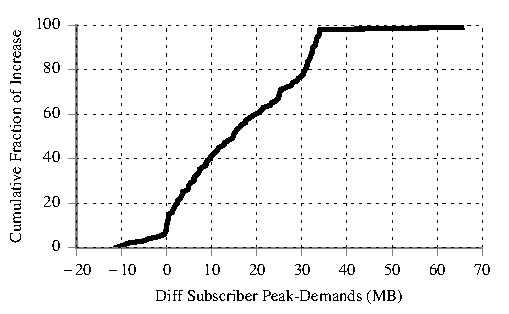
\includegraphics[width=\linewidth]{figures/cdf_diff_perc95_bytes_subsc-overall.pdf}
               \caption{Distribution of the difference between \treatment{} and \control{}
               peak traffic demands\label{fig:cdf-diff-perc95}}
\end{figure}


In Figure~\ref{fig:diff-peak-overall}, we plot the difference in
peak subscriber demands from the 
lowest peak to highest peak demanding subscribers in both groups.
As both groups had a different number of subscribers, we sort their peak demands
and difference the values at every percentile.
Comparing the lowest demanding 70\% subscribers of both groups, we
see that peak demand in \treatment{} is higher than the peak demand in \control{}.
Compared to figure~\ref{fig:CDF-data-rate-perc95}, these subscribers have a peak 
demand less than 200 MB.


Figure~\ref{fig:cdf-diff-perc95} shows the distribution of the difference in demands of the two
groups by percentile. There are 15\% subscribers in the \treatment{} 
that have peak demands have peak demands that are similar, or lower than the
equivalent 15\% of subscribers in \control{}. Figure~\ref{fig:diff-peak-overall} shows
that this group lies around between the 65 and 80 percentile demand. Figure~\ref{fig:CDF-data-rate-perc95}
shows that between the 65-80 percentile mark, subscribers had a demand between 
200~MB to 400~MB. For these subscribers in \treatment{}, the equivalent subscribers
in \control{} had demands upto 10~MB higher. 20\% of the differences between the peak
of the treatment group and the control group are higher than 30 MB. These subscribers
lie between the between 30\% and 50\% difference. Their a peak demands are between
between 40 -- 100 MB as part of the higher tier, and 10 -- 70 MB if they belong to
the lower tier.


The highest demanding subscribers in the \treatment{} (beyond 800 MB peak demand)
have demands 15~MB -- 30~MB more than the highest peak demanding subscribers
in \control{}.

For the upstream, 90\% of users in the treatment group consistently upload 2 MB
more traffic than the control group. The top 10\% of the highest demanding subscribers
in \treatment{} uploaded between 2~MB -- 10~MB more than the top 10\% of \control{}.

%\begin{figure}[t]
%\centering
%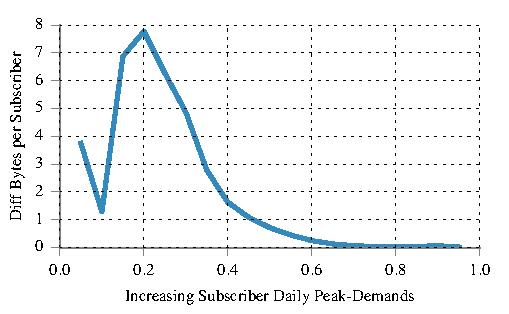
\includegraphics[width=\linewidth]{figures/diff_perc95_bytes_subsc-daily-normalized.pdf}
%               \caption{Ratio of the difference between \treatment{} and \control{}
%               in the daily peak traffic demand to the daily peak of the \control\label{fig:daily-ratio-perc95}}
%\end{figure}


\begin{figure}[t]
\begin{minipage}{1\linewidth}
\centering
%
% COMMENT OUT IF TAKING TOO MUCH SPACE
\begin{subfigure}[b]{1\linewidth}
 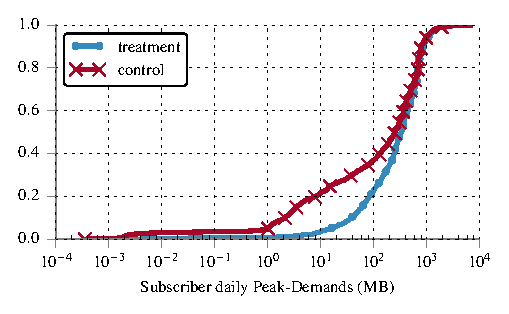
\includegraphics[width=\linewidth]{figures/cdf_peak_demand-daily.pdf}
                \caption{Peak (95\%) traffic demand per subscriber\label{fig:CDF-data-rate-daily-perc95}}
 \end{subfigure}
% 
% COMMENT OUT IF TAKING TOO MUCH SPACE
\begin{subfigure}[b]{.99\linewidth}
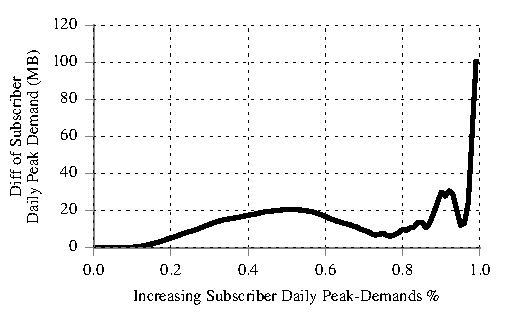
\includegraphics[width=\linewidth]{figures/diff_perc95_bytes_subsc-daily-overall_01.pdf}		%1 percentile
%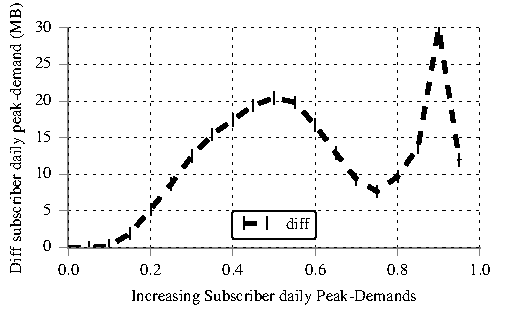
\includegraphics[width=\linewidth]{figures/diff_perc95_bytes_subsc-daily-overall.pdf}		%5 percentile
                \caption{Daily peak (95\%) per subscriber\label{fig:diff-peak-daily}}
\end{subfigure}
%
\end{minipage}
  \caption{Difference between peak-demands of subscribers from \treatment{} and
  \control{} groups. Subscribers were considered at every 5\% in each group.
  \label{fig:traffic-demand-daily}}
\end{figure}


On investigating further, we confirmed that this difference in the demands
of the lowest utilizing 50\% subscribers is also present daily.
Figure~\ref{fig:traffic-demand-daily} shows that when subscribers on the
lower tier had a daily peak demand under 600 MB, subscribers in the higher
tier had demands 5 -- 20 MB higher. This happens in 70\% of the instances.
On taking the ratio of the difference in demand, with the equivalent demand
of the lower tiers, we find that for 40\% of subscribers with low peak demands
in the control group, there are 40\% subscribers in the treatment group with
more than double their demands.
%(see Figure~\ref{fig:daily-ratio-perc95}).

There could be many reasons for this increase in demand for subscribers with
lower peak demands. One reason could be short term web activities (such as short videos,
web browsing) that have a slightly higher traffic demand. Such an increase in demand would
then be apparent during hours when users pursue such activities (mostly prime-time).
Another reason could be an increase in background traffic (such as software updates).
Studying the applications responsible for such behavioral changes in traffic demand is not
in the scope of our current work. However, an interesting question that arises is: when
does the demand increase the most throughout a day? Our analysis showed that the most
most subscribers reach within 95\% of daily maximum demand between 8:00 PM -- 12:00 AM.

% \begin{table}[h]
% \begin{tabular}{lllll}
%         &           & 1     & 2     & 3     \\
% Weekday & treatment & 21:45 & 00:00 & 23:30 \\
%         & control   & 22:30 & 22:15 & 00:00 \\
% Weekend & treatment & 23:30 & 23:45 & 14:30 \\
%         & control   & 22:30 & 21:30 &      
% \end{tabular}
% \end{table}